\documentclass[12pt, titlepage]{article}

\usepackage{fullpage}
\usepackage[round]{natbib}
\usepackage{multirow}
\usepackage{booktabs}
\usepackage{tabularx}
\usepackage{graphicx}
\usepackage{float}
\usepackage{longtable}
\usepackage{hyperref}
\hypersetup{
	colorlinks,
	citecolor=blue,
	filecolor=black,
	linkcolor=red,
	urlcolor=blue
}

%% Comments

\usepackage{color}

\newif\ifcomments\commentstrue %displays comments
%\newif\ifcomments\commentsfalse %so that comments do not display

\ifcomments
\newcommand{\authornote}[3]{\textcolor{#1}{[#3 ---#2]}}
\newcommand{\todo}[1]{\textcolor{red}{[TODO: #1]}}
\else
\newcommand{\authornote}[3]{}
\newcommand{\todo}[1]{}
\fi

\newcommand{\wss}[1]{\authornote{blue}{SS}{#1}} 
\newcommand{\plt}[1]{\authornote{magenta}{TPLT}{#1}} %For explanation of the template
\newcommand{\an}[1]{\authornote{cyan}{Author}{#1}}

%% Common Parts

\newcommand{\progname}{ProgName} % PUT YOUR PROGRAM NAME HERE
\newcommand{\authname}{Team \#, Team Name
\\ Student 1 name and macid
\\ Student 2 name and macid
\\ Student 3 name and macid
\\ Student 4 name and macid} % AUTHOR NAMES                  

\usepackage{hyperref}
    \hypersetup{colorlinks=true, linkcolor=blue, citecolor=blue, filecolor=blue,
                urlcolor=blue, unicode=false}
    \urlstyle{same}
                                


\newcounter{acnum}
\newcommand{\actheacnum}{AC\theacnum}
\newcommand{\acref}[1]{AC\ref{#1}}

\newcounter{ucnum}
\newcommand{\uctheucnum}{UC\theucnum}
\newcommand{\uref}[1]{UC\ref{#1}}

\newcounter{mnum}
\newcommand{\mthemnum}{M\themnum}
\newcommand{\mref}[1]{M\ref{#1}}

\begin{document}
	
	\title{Module Guide for \progname{}} 
	\author{\authname}
	\date{\today}
	
	\maketitle
	
	\pagenumbering{roman}
	
	\section{Revision History}
	
	\begin{tabularx}{\textwidth}{p{3cm}p{2cm}X}
		\toprule {\bf Date} & {\bf Version} & {\bf Notes}\\
		\midrule
		January 14 & 1.0 & Initial document created\\
		January 15 & 1.1 & Anticipated changes and hierarchy diagram added\\
		January 17 & 1.2 & Rest of document finished\\
		April 5 & 1.5 & Final document changes \\
		\bottomrule
	\end{tabularx}
	
	\newpage
	
	\section{Reference Material}
	
	This section records information for easy reference.
	
	\subsection{Abbreviations and Acronyms}
	
	\renewcommand{\arraystretch}{1.2}
	\begin{tabular}{l l} 
		\toprule		
		\textbf{symbol} & \textbf{description}\\
		\midrule 
		AC & Anticipated Change\\
		DAG & Directed Acyclic Graph \\
		M & Module \\
		MG & Module Guide \\
		OS & Operating System \\
		R & Requirement\\
		SC & Scientific Computing \\
		SRS & Software Requirements Specification\\
		HTTP & Hypertext Transfer Protocol, a protocol used to communicate over the internet\\
		TCP & Transmission Control Protocol, a protocol used to communicate over the internet\\
		PDF & A file type to display text and images\\
		\bottomrule
	\end{tabular}\\
	
	\newpage
	
	\tableofcontents
	
	\listoftables
	
	\listoffigures
	
	\newpage
	
	\pagenumbering{arabic}
	
	\section{Introduction}
	
	Decomposing a system into modules is a commonly accepted approach to developing
	software.  A module is a work assignment for a programmer or programming
	team~\citep{ParnasEtAl1984}.  We advocate a decomposition
	based on the principle of information hiding~\citep{Parnas1972a}.  This
	principle supports design for change, because the ``secrets'' that each module
	hides represent likely future changes.  Design for change is valuable in SC,
	where modifications are frequent, especially during initial development as the
	solution space is explored.  
	
	Our design follows the rules layed out by \citet{ParnasEtAl1984}, as follows:
	\begin{itemize}
		\item System details that are likely to change independently should be the
		secrets of separate modules.
		\item Each data structure is implemented in only one module.
		\item Any other program that requires information stored in a module's data
		structures must obtain it by calling access programs belonging to that module.
	\end{itemize}
	
	After completing the first stage of the design, the Software Requirements
	Specification (SRS), the Module Guide (MG) is developed~\citep{ParnasEtAl1984}. The MG
	specifies the modular structure of the system and is intended to allow both
	designers and maintainers to easily identify the parts of the software.  The
	potential readers of this document are as follows:
	
	\begin{itemize}
		\item New project members: This document can be a guide for a new project member
		to easily understand the overall structure and quickly find the
		relevant modules they are searching for.
		\item Maintainers: The hierarchical structure of the module guide improves the
		maintainers' understanding when they need to make changes to the system. It is
		important for a maintainer to update the relevant sections of the document
		after changes have been made.
		\item Designers: Once the module guide has been written, it can be used to
		check for consistency, feasibility, and flexibility. Designers can verify the
		system in various ways, such as consistency among modules, feasibility of the
		decomposition, and flexibility of the design.
	\end{itemize}
	
	The rest of the document is organized as follows. Section
	\ref{SecChange} lists the anticipated and unlikely changes of the software
	requirements. Section \ref{SecMH} summarizes the module decomposition that
	was constructed according to the likely changes. Section \ref{SecConnection}
	specifies the connections between the software requirements and the
	modules. Section \ref{SecMD} gives a detailed description of the
	modules. Section \ref{SecTM} includes two traceability matrices. One checks
	the completeness of the design against the requirements provided in the SRS. The
	other shows the relation between anticipated changes and the modules. Section
	\ref{SecUse} describes the use relation between modules.
	
	\section{Anticipated and Unlikely Changes} \label{SecChange}
	
	This section lists possible changes to the system. According to the likeliness
	of the change, the possible changes are classified into two
	categories. Anticipated changes are listed in Section \ref{SecAchange}, and
	unlikely changes are listed in Section \ref{SecUchange}.
	
	\subsection{Anticipated Changes} \label{SecAchange}
	
	Anticipated changes are the source of the information that is to be hidden
	inside the modules. Ideally, changing one of the anticipated changes will only
	require changing the one module that hides the associated decision. The approach
	adapted here is called design for
	change.
	
	\begin{description}
		
		\item[\refstepcounter{acnum} \actheacnum \label{ac1}:] The data structure and algorithm used to implement the virtual hardware.
		\item[\refstepcounter{acnum} \actheacnum \label{ac2}:]  How the components related to project editing will be displayed
		\item[\refstepcounter{acnum} \actheacnum \label{ac3}:]  How the current file being edited is displayed
		\item[\refstepcounter{acnum} \actheacnum \label{ac4}:]  The algorithm used to highlight syntax of the LaTeX code
		\refstepcounter{acnum}
		\item[\refstepcounter{acnum} \actheacnum \label{ac6}:]  How the list of files in the current project being edited will be displayed
		\item[\refstepcounter{acnum} \actheacnum \label{ac7}:]  The actions available on the file toolbar
		\item[\refstepcounter{acnum} \actheacnum \label{ac8}:]  Inputs needed to create a new file
		\item[\refstepcounter{acnum} \actheacnum \label{ac9}:]  Inputs needed to upload a file
		\item[\refstepcounter{acnum} \actheacnum \label{ac10}:]  Algorithm used for determine cursor position for all users currently editing the file
		\item[\refstepcounter{acnum} \actheacnum \label{ac11}:]  Algorithm used for highlighting text selected by other users
		\item[\refstepcounter{acnum} \actheacnum \label{ac12}:]  Algorithm used for synchronizing the file for all the users currently editing the file
		\item[\refstepcounter{acnum} \actheacnum \label{ac13}:]  The data type used to store files
		\item[\refstepcounter{acnum} \actheacnum \label{ac14}:]  The database queries used to save and retrieve file data
		\item[\refstepcounter{acnum} \actheacnum \label{ac15}:]  How the user will trigger the compilation of the LaTeX and download of the PDF file
		\item[\refstepcounter{acnum} \actheacnum \label{ac16}:]  How the user will view the PDF file
		\item[\refstepcounter{acnum} \actheacnum \label{ac17}:]  The algorithm used to compile the LaTeX code into a PDF
		\item[\refstepcounter{acnum} \actheacnum \label{ac18}:]  How the user will view and interact with the chat messages
		\item[\refstepcounter{acnum} \actheacnum \label{ac19}:]  The algorithm used to send and receive chat messages
		\item[\refstepcounter{acnum} \actheacnum \label{ac20}:]  The database queries used to save and retrieve chat data
		\item[\refstepcounter{acnum} \actheacnum \label{ac21}:]  The communication protocol used to communicate between users
		\item[\refstepcounter{acnum} \actheacnum \label{ac22}:]  The data type used for chat messages
		\item[\refstepcounter{acnum} \actheacnum \label{ac23}:]  How the instructions are displayed
		\item[\refstepcounter{acnum} \actheacnum \label{ac24}:]  How informational and actionable items related to project are displayed
		\item[\refstepcounter{acnum} \actheacnum \label{ac25}:]  How the project list are displayed
		\item[\refstepcounter{acnum} \actheacnum \label{ac26}:]  The methods used to delete a project
		\item[\refstepcounter{acnum} \actheacnum \label{ac27}:]  Different methods to create a project
		\item[\refstepcounter{acnum} \actheacnum \label{ac28}:]  Inputs needed to create a new project
		\item[\refstepcounter{acnum} \actheacnum \label{ac29}:]  Inputs needed to import a project
		\item[\refstepcounter{acnum} \actheacnum \label{ac30}:]  The different services offered in regards to creation, editing, and reading projects
		\item[\refstepcounter{acnum} \actheacnum \label{ac31}:]  The algorithm used to fetch project data from the database
		\item[\refstepcounter{acnum} \actheacnum \label{ac32}:]  The format of project data
		\item[\refstepcounter{acnum} \actheacnum \label{ac33}:]  The user interface to interact with GitHub
		\item[\refstepcounter{acnum} \actheacnum \label{ac34}:]  The user interface to login and logout with GitHub
		\item[\refstepcounter{acnum} \actheacnum \label{ac35}:]  The algorithm to authenticate the user with GitHub
		\item[\refstepcounter{acnum} \actheacnum \label{ac36}:]  The functions used to save and retrieve authentication data for a user
		\item[\refstepcounter{acnum} \actheacnum \label{ac37}:]  The datatype for authenticating a user
		
		\refstepcounter{acnum}
		\refstepcounter{acnum}
		% \item[\refstepcounter{acnum} \actheacnum \label{ac49}:] % \item[Secrets:] The algorithm to retrieve all the remote changes on GitHub
		
		% \item[\refstepcounter{acnum} \actheacnum \label{ac50}:] % \item[Secrets:] How the project details are updated in the database
		
		\item[\refstepcounter{acnum} \actheacnum \label{ac51}:]  How data is stored
	\end{description}
	
	\subsection{Unlikely Changes} \label{SecUchange}
	
	The module design should be as general as possible. However, a general system is
	more complex. Sometimes this complexity is not necessary. Fixing some design
	decisions at the system architecture stage can simplify the software design. If
	these decision should later need to be changed, then many parts of the design
	will potentially need to be modified. Hence, it is not intended that these
	decisions will be changed.
	
	\begin{description}
		\item[\refstepcounter{ucnum} \uctheucnum \label{uc1}:] Input using mouse and keyboard
		\item[\refstepcounter{ucnum} \uctheucnum \label{uc2}:] Output using computer monitor. Limited but existing functionality for mobile devices
		\item[\refstepcounter{ucnum} \uctheucnum \label{uc2}:] Utilizing GitHub for version control
		\item[\refstepcounter{ucnum} \uctheucnum \label{uc2}:] Using access tokens and JWTs to authentication and security
	\end{description}
	
	\section{Module Hierarchy} \label{SecMH}
	
	This section provides an overview of the module design. Modules are summarized
	in a hierarchy decomposed by secrets in Table \ref{TblMH}. The modules listed
	below, which are leaves in the hierarchy tree, are the modules that will
	actually be implemented.
	
	
	
	\begin{description}
		% example:
		% \item [\refstepcounter{mnum} \mthemnum \label{mHH}:] Hardware-Hiding Module
		\item [\refstepcounter{mnum} \mthemnum: \label{m1}] Hardware-Hiding Module
		\item [\refstepcounter{mnum} \mthemnum: \label{m2}] Project Editing Module
		\item [\refstepcounter{mnum} \mthemnum: \label{m3}] Editor Module
		\item [\refstepcounter{mnum} \mthemnum: \label{m4}] Syntax Highlighting Module
		\refstepcounter{mnum}
		\item [\refstepcounter{mnum} \mthemnum: \label{m6}] File List Module
		\item [\refstepcounter{mnum} \mthemnum: \label{m7}] File Toolbar Module
		\item [\refstepcounter{mnum} \mthemnum: \label{m8}] New File Module
		\item [\refstepcounter{mnum} \mthemnum: \label{m9}] Upload File Module
		\item [\refstepcounter{mnum} \mthemnum: \label{m10}] User Cursors Module
		\item [\refstepcounter{mnum} \mthemnum: \label{m11}] Text Highlighting Module
		\item [\refstepcounter{mnum} \mthemnum: \label{m12}] File Synchronization Module
		\item [\refstepcounter{mnum} \mthemnum: \label{m13}] File Services Module
		\item [\refstepcounter{mnum} \mthemnum: \label{m14}] File Database Interface Module
		\item [\refstepcounter{mnum} \mthemnum: \label{m15}] PDF Module
		\item [\refstepcounter{mnum} \mthemnum: \label{m16}] PDF Renderer Module
		\item [\refstepcounter{mnum} \mthemnum: \label{m17}] PDF Compiler Module
		\item [\refstepcounter{mnum} \mthemnum: \label{m18}] Chat Module
		\item [\refstepcounter{mnum} \mthemnum: \label{m19}] Chat Services Module
		\item [\refstepcounter{mnum} \mthemnum: \label{m20}] Chat Database Interface Module
		\item [\refstepcounter{mnum} \mthemnum: \label{m21}] Chat Socket Module
		\item [\refstepcounter{mnum} \mthemnum: \label{m22}] Chat Data Module
		\item [\refstepcounter{mnum} \mthemnum: \label{m23}] Instructions View Module
		\item [\refstepcounter{mnum} \mthemnum: \label{m24}] Projects
		\item [\refstepcounter{mnum} \mthemnum: \label{m25}] Project List
		\item [\refstepcounter{mnum} \mthemnum: \label{m26}] Project Deletion
		\item [\refstepcounter{mnum} \mthemnum: \label{m27}] Project Creation
		\item [\refstepcounter{mnum} \mthemnum: \label{m28}] New Project
		\item [\refstepcounter{mnum} \mthemnum: \label{m29}] Import Project
		\item [\refstepcounter{mnum} \mthemnum: \label{m30}] Project Services
		\item [\refstepcounter{mnum} \mthemnum: \label{m31}] Project Database Interface
		\item [\refstepcounter{mnum} \mthemnum: \label{m32}] Project Data
		\item [\refstepcounter{mnum} \mthemnum: \label{m33}] GitHub Module
		\item [\refstepcounter{mnum} \mthemnum: \label{m34}] GitHub Services Module
		\item [\refstepcounter{mnum} \mthemnum: \label{m35}] Authentication Module
		\item [\refstepcounter{mnum} \mthemnum: \label{m36}] Auth Service Module
		\item [\refstepcounter{mnum} \mthemnum: \label{m37}] Auth Database Interface Module
		\item [\refstepcounter{mnum} \mthemnum: \label{m38}] Auth Data Module
		\item [\refstepcounter{mnum} \mthemnum: \label{m39}] MongoDB
		\item [\refstepcounter{mnum} \mthemnum: \label{m40}] File Data
	\end{description}
	
	
	\begin{table}[H]
		\centering
		\scriptsize\begin{longtable}{p{0.3\textwidth} p{0.6\textwidth}}
			\caption{Module Hierarchy} \\
			\toprule
			\textbf{Level 1} & \textbf{Level 2}\\
			\midrule
			
			{Hardware-Hiding Module} & ~ \\
			\midrule
			
			\multirow{37}{0.3\textwidth}{Behaviour-Hiding Module}  & Project Editing Module \\
			& Editor Module \\
			& Syntax Highlighting Module \\
			& File List Module \\
			& File Toolbar Module \\
			& New File Module \\
			& Upload File Module \\
			& User Cursors Module \\
			& Text Highlighting Module \\
			& File Synchronization Module \\
			& File Services Module \\
			& File Database Interface Module \\
			& PDF Module \\
			& PDF Renderer Module \\
			& PDF Compiler Module \\
			& Chat Module \\
			& Chat Services Module \\
			& Chat Database Interface Module \\
			& Chat Socket Module \\
			& Instructions View Module \\
			& Projects Module \\
			& Project List Module \\
			& Project Deletion Module \\
			& Project Creation Module \\
			& New Project Module \\
			& Import Project Module \\
			& Project Services Module \\
			& Project Database Interface Module \\
			& GitHub Module \\
			& GitHub Services Module \\
			& Authentication Module \\
			& Auth Service Module \\
			& Auth Database Interface Module \\
			\midrule
			\newpage
			\multirow{1}{0.3\textwidth}{Software Decision Module} & \\
			& File Data Module \\
			& Chat Data Module \\
			& Project Data Module \\
			& Auth Data Module \\
			& MongoDB Module \\
			\bottomrule
			
		\end{longtable}
		
		\label{TblMH}
	\end{table}
	\normalsize
	
	\section{Connection Between Requirements and Design} \label{SecConnection}
	
	The design of the system is intended to satisfy the requirements developed in
	the SRS. In this stage, the system is decomposed into modules. The connection
	between requirements and modules is listed in Table~\ref{TblRT1} and ~\ref{TblRT}.
	
	\section{Module Decomposition} \label{SecMD}
	
	Modules are decomposed according to the principle of ``information hiding''
	proposed by \citet{ParnasEtAl1984}. The \emph{Secrets} field in a module
	decomposition is a brief statement of the design decision hidden by the
	module. The \emph{Services} field specifies \emph{what} the module will do
	without documenting \emph{how} to do it. For each module, a suggestion for the
	implementing software is given under the \emph{Implemented By} title. If the
	entry is \emph{OS}, this means that the module is provided by the operating
	system or by standard programming language libraries.  \emph{\progname{}} means the
	module will be implemented by the \progname{} software.
	
	Only the leaf modules in the hierarchy have to be implemented. If a dash
	(\emph{--}) is shown, this means that the module is not a leaf and will not have
	to be implemented.
	
	\subsection{Hardware Hiding Modules (\mref{m1})}
	
	\begin{description}
		\item[Secrets:]The data structure and algorithm used to implement the virtual hardware.
		\item[Services:]Serves as a virtual hardware used by the rest of the
		system. This module provides the interface between the hardware and the
		software. So, the system can use it to display outputs or to accept inputs.
		\item[Implemented By:] OS
	\end{description}
	
	\subsection{Behaviour-Hiding Module}
	
	
	\subsubsection{Project Editing Module (\mref{m2})}
	
	\begin{description}
		\item[Secrets:] How the components related to project editing will be displayed
		\item[Services:] Displays the various components of project editing which are the file editor, file list, PDF output and information about the project being edited
		\item[Implemented By:] UnderTree
		\item[Type of Module:] Abstract Object
	\end{description}
	
	\subsubsection{Editor Module (\mref{m3})}
	
	\begin{description}
		\item[Secrets:] How the current file being edited is displayed
		\item[Services:] Displays the content of the current file being edited and details about that file
		\item[Implemented By:] UnderTree
		\item[Type of Module:] Abstract Object
	\end{description}
	
	\subsubsection{Syntax Highlight Module (\mref{m4})}
	
	\begin{description}
		\item[Secrets:] The algorithm used to highlight syntax of the LaTeX code
		\item[Services:] T module will highlight the text based on LaTeX syntax
		\item[Implemented By:] Highlight.js
		\item[Type of Module:] Library
	\end{description}
	
	% \subsubsection{Spelling Error Module (\mref{m5})}
	
	% \begin{description}
		% \item[Secrets:] The algorithm used to highlight grammar and spelling errors of the LaTeX code
		% \item[Services:] Given input LaTeX code, this module will highlight the grammar and spelling errors in the LaTeX code
		% \item[Implemented By:] BeyondGrammar
		% \item[Type of Module:] Library
		% \end{description}
	
	\subsubsection{File List Module (\mref{m6})}
	
	\begin{description}
		\item[Secrets:] How the list of files in the current project being edited will be displayed
		\item[Services:] Displays the list of files in the current project and allows the user to open them in the editor, rename or delete a file
		\item[Implemented By:] UnderTree
		\item[Type of Module:] Abstract Object
	\end{description}
	
	\subsubsection{File Toolbar Module (\mref{m7})}
	
	\begin{description}
		\item[Secrets:] The actions available on the file toolbar
		\item[Services:] Allows for actions regarding file such as adding a new file or uploading a new file
		\item[Implemented By:] UnderTree
		\item[Type of Module:] Abstract Object
	\end{description}
	
	\subsubsection{New File Module (\mref{m8})}
	
	\begin{description}
		\item[Secrets:] Inputs needed to create a new file
		\item[Services:] Creates a new file in the project using name and extension as input
		\item[Implemented By:] UnderTree
		\item[Type of Module:] Abstract Object
	\end{description}
	
	\subsubsection{Upload File Module (\mref{m9})}
	
	\begin{description}
		\item[Secrets:] Inputs needed to upload a file
		\item[Services:] Uploads a local file to the current project being edited
		\item[Implemented By:] UnderTree
		\item[Type of Module:] Abstract Object
	\end{description}
	
	\subsubsection{User Cursors Module (\mref{m10})}
	
	\begin{description}
		\item[Secrets:] Algorithm used for determine cursor position for all users currently editing the file
		\item[Services:] Gives the current cursor position for the a spcecifc user in the editor
		\item[Implemented By:] YJS
		\item[Type of Module:] Library
	\end{description}
	
	\subsubsection{Text Highlighting Module (\mref{m11})}
	
	\begin{description}
		\item[Secrets:] Algorithm used for highlighting text selected by other users
		\item[Services:] Gives the current highlighted text for the a specific user in the editor
		\item[Implemented By:] YJS
		\item[Type of Module:] Library
	\end{description}
	
	\subsubsection{File Synchronization Module (\mref{m12})}
	
	\begin{description}
		\item[Secrets:] Algorithm used for synchronizing the file for all the users currently editing the file
		\item[Services:] Displays the file with all the changes made by different collaborators up until that current instance of time
		\item[Implemented By:] \href{https://docs.yjs.dev/}{YJS}
		\item[Type of Module:] Abstract Object
	\end{description}
	
	\subsubsection{File Services (\mref{m13})}
	
	\begin{description}
		\item[Secrets:] The data type used to store files
		\item[Services:] Offers services for creating new file, editing existing files, deleting a file, and getting information about one or more files
		\item[Implemented By:] UnderTree
		\item[Type of Module:] Abstract Object
	\end{description}
	
	\subsubsection{File Database Interface Module (\mref{m14})}
	
	\begin{description}
		\item[Secrets:] The database queries used to save and retrieve file data
		\item[Services:] This module is responsible for providing the functions to make the relevant queries to save and retrieve file data
		\item[Implemented By:] UnderTree
		\item[Type of Module:] Abstract Object
	\end{description}
	
	\subsubsection{PDF Module (\mref{m15})}
	
	\begin{description}
		\item[Secrets:] How the user will trigger the compilation of the LaTeX and download of the PDF file
		\item[Services:] This module is responsible for allowing the user to download, and start the compilation for the LaTeX to PDF
		\item[Implemented By:] UnderTree
		\item[Type of Module:] Abstract Object
	\end{description}
	
	\subsubsection{PDF Renderer Module (\mref{m16})}
	
	\begin{description}
		\item[Secrets:] How the user will view the PDF file
		\item[Services:] This module is responsible for allowing the user to view the LaTeX file
		\item[Implemented By:] \href{https://mozilla.github.io/pdf.js/examples/}{PDF.js}
		\item[Type of Module:] Abstract Object
	\end{description}
	
	\subsubsection{PDF Compiler Module (\mref{m17})}
	
	\begin{description}
		\item[Secrets:] The algorithm used to compile the LaTeX code into a PDF
		\item[Services:] Upon getting a request from the PDF module to compile the PDF this module is used to convert the LaTeX code into a PDF which the user can view
		\item[Implemented By:] \href{https://www.npmjs.com/package/node-LaTeX}{node-LaTeX}
		\item[Type of Module:] Library
	\end{description}
	
	\subsubsection{Chat Module (\mref{m18})}
	
	\begin{description}
		\item[Secrets:] How the user will view and interact with the chat messages
		\item[Services:] This module is responsible for allowing the user to view and input chat messages
		\item[Implemented By:] UnderTree
		\item[Type of Module:] Abstract Object
	\end{description}
	
	\subsubsection{Chat Services Module (\mref{m19})}
	
	\begin{description}
		\item[Secrets:] The algorithm used to send and receive chat messages
		\item[Services:] This module is responsible for sending and receiving chat messages between users
		\item[Implemented By:] UnderTree
		\item[Type of Module:] Abstract Object
	\end{description}
	
	\subsubsection{Chat Database Interface Module (\mref{m20})}
	
	\begin{description}
		\item[Secrets:] The database queries used to save and retrieve chat data
		\item[Services:] This module is responsible for providing the functions needed to make the relevant queries to save and retrieve chat data
		\item[Implemented By:] UnderTree
		\item[Type of Module:] Abstract Object
	\end{description}
	
	\subsubsection{Chat Socket Module (\mref{m21})}
	
	\begin{description}
		\item[Secrets:] The communication protocol used to communicate between users
		\item[Services:] This module is responsible for providing the web sockets needed to communicate between users in a synchronized manner
		\item[Implemented By:] \href{https://socket.io/docs/v4/}{Socket.IO}
		\item[Type of Module:] Abstract Object
	\end{description}
	
	\subsubsection{Instructions View Module (\mref{m23})}
	
	\begin{description}
		\item[Secrets:] How the instructions are displayed
		\item[Services:] This module is responsible for allowing users to open and close as well as view the instructions in an organized manner
		\item[Implemented By:] UnderTree
		\item[Type of Module:] Abstract Object
	\end{description}
	
	\subsubsection{Projects (\mref{m24})}
	
	\begin{description}
		\item[Secrets:] How informational and actionable items related to project are displayed
		\item[Services:] This module displays the project list, allows the creation of new project and also displays other items related to projects
		\item[Implemented By:] UnderTree
		\item[Type of Module:] Abstract Object
	\end{description}
	
	\subsubsection{Project List (\mref{m25})}
	
	\begin{description}
		\item[Secrets:] How the project list are displayed
		\item[Services:] This module displays a list of all the available projects to the user which can be opened or deleted
		\item[Implemented By:] UnderTree
		\item[Type of Module:] Abstract Object
	\end{description}
	
	\subsubsection{Project Deletion (\mref{m26})}
	
	\begin{description}
		\item[Secrets:] The methods used to delete a project
		\item[Services:] Allows users to delete the project
		\item[Implemented By:] UnderTree
		\item[Type of Module:] Abstract Object
	\end{description}
	
	\subsubsection{Project Creation (\mref{m27})}
	
	\begin{description}
		\item[Secrets:] The modal that contains the different methods to create a project (creation or import)
		\item[Services:] Presents a user interface for users to choose how they want to create their project either from scratch or importing a pre-existing project
		\item[Implemented By:] UnderTree
		\item[Type of Module:] Abstract Object
	\end{description}
	
	\subsubsection{New Project (\mref{m28})}
	
	\begin{description}
		\item[Secrets:] Inputs needed to create a new project
		\item[Services:] Presents a user interface for users to create, title and add contributors to a new project from scratch
		\item[Implemented By:] UnderTree
		\item[Type of Module:] Abstract Object
	\end{description}
	
	\subsubsection{Import Project (\mref{m29})}
	
	\begin{description}
		\item[Secrets:] Inputs needed to import a project
		\item[Services:] This module provides a user interface for the user to import pre-existing projects into UnderTree
		\item[Implemented By:] UnderTree
		\item[Type of Module:] Abstract Object
	\end{description}
	
	\subsubsection{Project Services (\mref{m30})}
	
	\begin{description}
		\item[Secrets:] The different services offered in regards to creation, editing, and reading projects
		\item[Services:] Offers services for creating new project, editing existing project, deleting a project, and getting information about one or more projects
		\item[Implemented By:] UnderTree
		\item[Type of Module:] Abstract Object
	\end{description}
	
	\subsubsection{Project Database Interface (\mref{m31})}
	
	\begin{description}
		\item[Secrets:] The algorithm used to fetch project data from the database
		\item[Services:] Offers service to modify project data in the database
		\item[Implemented By:] UnderTree
		\item[Type of Module:] Abstract Object
	\end{description}
	
	\subsubsection{GitHub Module (\mref{m33})}
	
	\begin{description}
		\item[Secrets:] The logic to display the GitHub buttons and modal
		\item[Services:] Responsible for receiving the user data.
		\item[Implemented By:] UnderTree
		\item[Type of Module:] Abstract Object
	\end{description}
	
	\subsubsection{GitHub Services Module (\mref{m34})}
	
	\begin{description}
		\item[Secrets:] The algorithm to communicate with GitHub API
		\item[Services:] Responsible for performing the GitHub operations.
		\item[Implemented By:] UnderTree
		\item[Type of Module:] Abstract Object
	\end{description}
	
	\subsubsection{Authentication Module (\mref{m35})}
	
	\begin{description}
		\item[Secrets:] The algorithm to access different authorization modules
		\item[Services:] This module determines which module to use based on the action the user is performing
		\item[Implemented By:] UnderTree
		\item[Type of Module:] Abstract Object
	\end{description}
	
	\subsubsection{Auth Service Module (\mref{m36})}
	
	\begin{description}
		\item[Secrets:] The algorithm to handle the HTTPS requests and authentication
		\item[Services:] This module contains the main logic for authentication with GitHub
		\item[Implemented By:] UnderTree
		\item[Type of Module:] Abstract Object
	\end{description}
	
	\subsubsection{Auth Database Interface Module (\mref{m37})}
	
	\begin{description}
		\item[Secrets:] The algorithm to save user authentication data
		\item[Services:] This module serves as a wrapper and makes queries with the database MongoDB.
		\item[Implemented By:] UnderTree
		\item[Type of Module:] Abstract Object
	\end{description}
	
	\subsection{Software Decision Module}
	
	\subsubsection{File Data Module (\mref{m40})}
	
	\begin{description}
		\item[Secrets:] The data type used for files
		\item[Services:] This module stores the datatype that will be used to represent file system in each project
		\item[Implemented By:] UnderTree
		\item[Type of Module:] Record
	\end{description}
	
	\subsubsection{Chat Data Module (\mref{m22})}
	
	\begin{description}
		\item[Secrets:] The data type used for chat messages
		\item[Services:] This module stores the datatype that will be used to represent chat messages
		\item[Implemented By:] UnderTree
		\item[Type of Module:] Record
	\end{description}
	
	\subsubsection{Project Data (\mref{m32})}
	
	\begin{description}
		\item[Secrets:] The format of project data
		\item[Services:] Represents the format for the project data
		\item[Implemented By:] UnderTree
		\item[Type of Module:] Record
	\end{description}
	
	\subsubsection{Auth Data Module (\mref{m38})}
	
	\begin{description}
		\item[Secrets:] The data types in authentication are declared here
		\item[Services:] This module allows for the storing and retrieving of several key data structures that will be used for authentication.
		\item[Implemented By:] UnderTree
		\item[Type of Module:] Record
	\end{description}
	
	\subsubsection{MongoDB Module (\mref{m39})}
	
	\begin{description}
		\item[Secrets:] How data is stored
		\item[Services:] Allows you to retrieve and store data from the database
		\item[Implemented By:] MongoDB
		\item[Type of Module:] Library
	\end{description}
	
	\newpage
	
	\section{Traceability Matrix} \label{SecTM}
	
	This section shows two traceability matrices: between the modules and the
	requirements and between the modules and the anticipated changes.
	
	% the table should use mref, the requirements should be named, use something
	% like fref
	% \begin{table}[H]
		% \centering
		\begin{longtable}{p{0.2\textwidth} p{0.6\textwidth}}
			\caption{Trace Between Functional Requirements and Modules}
			\label{TblRT1} \\
			\toprule
			\textbf{Req.} & \textbf{Modules}\\
			\midrule
			FR1 & \mref{m23} \\
			FR2 & \mref{m23} \\
			FR3 & \mref{m33}, \mref{m34}, \mref{m35}, \mref{m36} \\
			FR4 & \mref{m33}, \mref{m34}, \mref{m35}, \mref{m36} \\
			FR5 & \mref{m24}, \mref{m27}, \mref{m28}, \mref{m30}, \mref{m31}, \mref{m32} \\
			FR6 & \mref{m24}, \mref{m27}, \mref{m28}, \mref{m30}, \mref{m31}, \mref{m32} \\
			FR7 & \mref{m33}, \mref{m34}, \mref{m37}, \mref{m38}, \mref{m39}\\
			FR8 & \mref{m24}, \mref{m27}, \mref{m29}, \mref{m30}, \mref{m31}, \mref{m32} \\
			FR9 & \mref{m30}, \mref{m31}, \mref{m32}, \mref{m33}, \mref{m51} \\
			FR10 & \mref{m30}, \mref{m31}, \mref{m32}, \mref{m33} \\
			FR11 & \mref{m26}, \mref{m30}, \mref{m31}, \mref{m32}, \mref{m39} \\
			FR12 & \mref{m26}, \mref{m30}, \mref{m31}, \mref{m32}, \mref{m39} \\
			FR13 & \mref{m24}, \mref{m25}, \mref{m30}, \mref{m31}, \mref{m32}, \mref{m39} \\
			FR14 & \mref{m24}, \mref{m25}, \mref{m30}, \mref{m31}, \mref{m32}, \mref{m39} \\
			FR15 & \mref{m24}, \mref{m25}, \mref{m30}, \mref{m31}, \mref{m32}, \mref{m39} \\
			FR16 & \mref{m2}, \mref{m25}, \mref{m30}, \mref{m31}, \mref{m32}, \mref{m33}, \mref{m35}, \mref{m39} \\
			FR17 & \mref{m2}, \mref{m25}, \mref{m30}, \mref{m31}, \mref{m32}, \mref{m33}, \mref{m35}, \mref{m39} \\
			FR18 & \mref{m6}, \mref{m13}, \mref{m14}\\
			FR19 & \mref{m6}, \mref{m13}, \mref{m14} \\
			FR20 & \mref{m3}, \mref{m10} \\
			FR21 & \mref{m3}, \mref{m12} \\
			FR22 & \mref{m3}, \mref{m4} \\
			FR23 & \mref{m3} \\
			\hline 
			\newpage
			\hline
			FR24 & \mref{m7}, \mref{m8} \\
			FR25 & \mref{m7}, \mref{m8} \\
			FR26 & \mref{m6}, \mref{m13}, \mref{m14}, \mref{40}\\
			FR27 & \mref{m7}, \mref{m9}\\
			FR28 & \mref{m6}, \mref{m13}, \mref{m14}\\
			FR29 & \mref{m6}, \mref{m7}\\
			FR30 & \mref{m6}, \mref{m13}, \mref{m14}\\
			FR31 & \mref{m6} \\
			FR32 & \mref{m13}, \mref{m14}\\
			FR33 & \mref{m13}, \mref{m14}\\
			FR34 & \mref{m3}\\
			FR35 & \mref{m3}, \mref{m13}, \mref{m14}, \mref{m38} \\
			FR36 & \mref{m13}, \mref{m14}, \mref{m17} \\
			FR37 & \mref{m2}, \mref{m15} \\
			FR38 & \mref{m13}, \mref{m14},  \mref{m17} \\
			FR39 & \mref{m2}, \mref{m15}, \mref{m16} \\
			FR40 & \mref{m2},\mref{m45} \\
			FR41 & \mref{m2},\mref{m45} \\
			FR42 & \mref{m2} \\
			FR43 & \mref{m18} \\
			FR44 & \mref{m18}, \mref{m19}, \mref{m20}, \mref{m21}, \mref{m22} \\
			FR45 & \mref{m33}, \mref{m35} \\
			FR46 & \mref{m33}, \mref{m35} \\
			FR47 & \mref{m33}, \mref{m35} \\
			\bottomrule
		\end{longtable}
		% \end{table}
	\newpage
	
	
	\begin{longtable}{p{0.2\textwidth} p{0.6\textwidth}}
		\caption{Trace Between Nonfunctional Requirements and Modules}
		\label{TblRT} \\
		\toprule
		\textbf{Req.} & \textbf{Modules}\\
		\midrule
		NFR1 & \mref{m2}, \mref{m3}, \mref{m18}, \mref{m23}, \mref{m24} \\
		NFR1 & \mref{m2}, \mref{m3}, \mref{m18}, \mref{m23}, \mref{m24} \\
		NFR3 & \mref{m2}, \mref{m3}, \mref{m18}, \mref{m23}, \mref{m24} \\
		NFR4 & \mref{m33}, \mref{m34}, \mref{m35}, \mref{m35} \\
		NFR5 & \mref{m2}, \mref{m3}, \mref{m18}, \mref{m23}, \mref{m24} \\
		NFR6 & \mref{m24}, \mref{m27}, \mref{m28}, \mref{m30}, \mref{m31}, \mref{m32} \\
		NFR7 & \mref{m33}, \mref{m34}, \mref{m35}, \mref{m36}, \mref{m37}\\
		NFR8 & \mref{m2}, \mref{m3}, \mref{m18}, \mref{m23}, \mref{m24} \\
		NFR9 & \mref{m30}, \mref{m31}, \mref{m32}, \mref{m33}, \mref{m39} \\
		NFR10 & \mref{m30}, \mref{m31}, \mref{m32}, \mref{m33} \\
		NFR11 & \mref{m26}, \mref{m30}, \mref{m31}, \mref{m32}, \mref{m39} \\
		NFR12 & \mref{m26}, \mref{m30}, \mref{m31}, \mref{m32}, \mref{m39} \\
		NFR13 & \mref{m24}, \mref{m25}, \mref{m30}, \mref{m31}, \mref{m32}, \mref{m39} \\
		NFR14 & \mref{m24}, \mref{m25}, \mref{m30}, \mref{m31}, \mref{m32}, \mref{m39} \\
		NFR15 & \mref{m24}, \mref{m25}, \mref{m30}, \mref{m31}, \mref{m32}, \mref{m39} \\
		NFR16 & \mref{m2}, \mref{m25}, \mref{m30}, \mref{m31}, \mref{m32}, \mref{m33}, \mref{m34}, \mref{m39} \\
		NFR17 & \mref{m2}, \mref{m25}, \mref{m30}, \mref{m31}, \mref{m32}, \mref{m33}, \mref{m34}, \mref{m39} \\
		NFR18 & \mref{m6}, \mref{m13}, \mref{m14}\\
		NFR19 & \mref{m6}, \mref{m13}, \mref{m14} \\
		NFR20 & \mref{m3}, \mref{m10} \\
		NFR21 & \mref{m3}, \mref{m12} \\
		NFR22 & \mref{m3}, \mref{m4} \\
		NFR23 & \mref{m3} \\
		\hline 
		\newpage
		\hline
		NFR24 & \mref{m7}, \mref{m8} \\
		NFR25 & \mref{m7}, \mref{m8} \\
		NFR26 & \mref{m6}, \mref{m13}, \mref{m14}\\
		NFR27 & \mref{m7}, \mref{m9}\\
		NFR28 & \mref{m6}, \mref{m13}, \mref{m14}\\
		NFR29 & \mref{m6}, \mref{m7}\\
		NFR30 & \mref{m6}, \mref{m13}, \mref{m14}\\
		NFR31 & \mref{m2}, \mref{m3}, \mref{m18}, \mref{m23}, \mref{m24} \\
		NFR32 & \mref{m13}, \mref{m14}\\
		NFR33 & \mref{m13}, \mref{m14}\\
		NFR34 & \mref{m2}, \mref{m3}, \mref{m18}, \mref{m23}, \mref{m24} \\
		NFR35 & \mref{m3}, \mref{m13}, \mref{m14} \\
		NFR36 & \mref{m13}, \mref{m14}, \mref{m17} \\
		NFR37 & \mref{m2}, \mref{m15} \\
		NFR38 & \mref{m13}, \mref{m14},  \mref{m17} \\
		NFR39 & \mref{m2}, \mref{m15}, \mref{m16} \\
		NFR40 & \mref{m2},\mref{m38} \\
		NFR44 & \mref{m18}, \mref{m19}, \mref{m20}, \mref{m21}, \mref{m22} \\
		\bottomrule
	\end{longtable}
	% \end{table}
\newpage



% \begin{table}[H]
	% \centering
	\begin{longtable}{p{0.2\textwidth} p{0.6\textwidth}}
		\caption{Trace Between Anticipated Changes and Modules}
		\label{TblACT}\\
		\toprule
		\textbf{AC} & \textbf{Modules}\\
		\midrule
		\acref{ac1} & \mref{m1}\\
		\acref{ac2} & \mref{m2}\\
		\acref{ac3} & \mref{m3}\\
		\acref{ac4} & \mref{m4}\\
		% \acref{ac5} & \mref{m5}\\
		\acref{ac6} & \mref{m6}\\
		\acref{ac7} & \mref{m7}\\
		\acref{ac8} & \mref{m8}\\
		\acref{ac9} & \mref{m9}\\
		\acref{ac10} & \mref{m10}\\
		\acref{ac11} & \mref{m11}\\
		\acref{ac12} & \mref{m12}\\
		\acref{ac13} & \mref{m13}\\
		\acref{ac14} & \mref{m14}\\
		\acref{ac15} & \mref{m15}\\
		\acref{ac16} & \mref{m16}\\
		\acref{ac17} & \mref{m17}\\
		\acref{ac18} & \mref{m18}\\
		\acref{ac19} & \mref{m19}\\
		\acref{ac20} & \mref{m20}\\
		\acref{ac21} & \mref{m21}\\
		\acref{ac22} & \mref{m22}\\
		\acref{ac23} & \mref{m23}\\
		\acref{ac24} & \mref{m24}\\
		\acref{ac25} & \mref{m25}\\
		\acref{ac26} & \mref{m26}\\
		\acref{ac27} & \mref{m27}\\
		\acref{ac28} & \mref{m28}\\
		\acref{ac29} & \mref{m29}\\
		\acref{ac30} & \mref{m30}\\
		\acref{ac31} & \mref{m31}\\
		\acref{ac32} & \mref{m32}\\
		\acref{ac33} & \mref{m33}\\
		\acref{ac34} & \mref{m34}\\
		\acref{ac35} & \mref{m35}\\
		\acref{ac36} & \mref{m36}\\
		\acref{ac37} & \mref{m37}\\
		
		\bottomrule
	\end{longtable}
	% \end{table}

\section{Use Hierarchy Between Modules} \label{SecUse}

In this section, the uses hierarchy between modules is
provided. \citet{Parnas1978} said of two programs A and B that A {\em uses} B if
correct execution of B may be necessary for A to complete the task described in
its specification. That is, A {\em uses} B if there exist situations in which
the correct functioning of A depends upon the availability of a correct
implementation of B.  Figure \ref{FigUH} illustrates the use relation between
the modules. It can be seen that the graph is a directed acyclic graph
(DAG). Each level of the hierarchy offers a testable and usable subset of the
system, and modules in the higher level of the hierarchy are essentially simpler
because they use modules from the lower levels.

\begin{figure}[H]
	\centering
	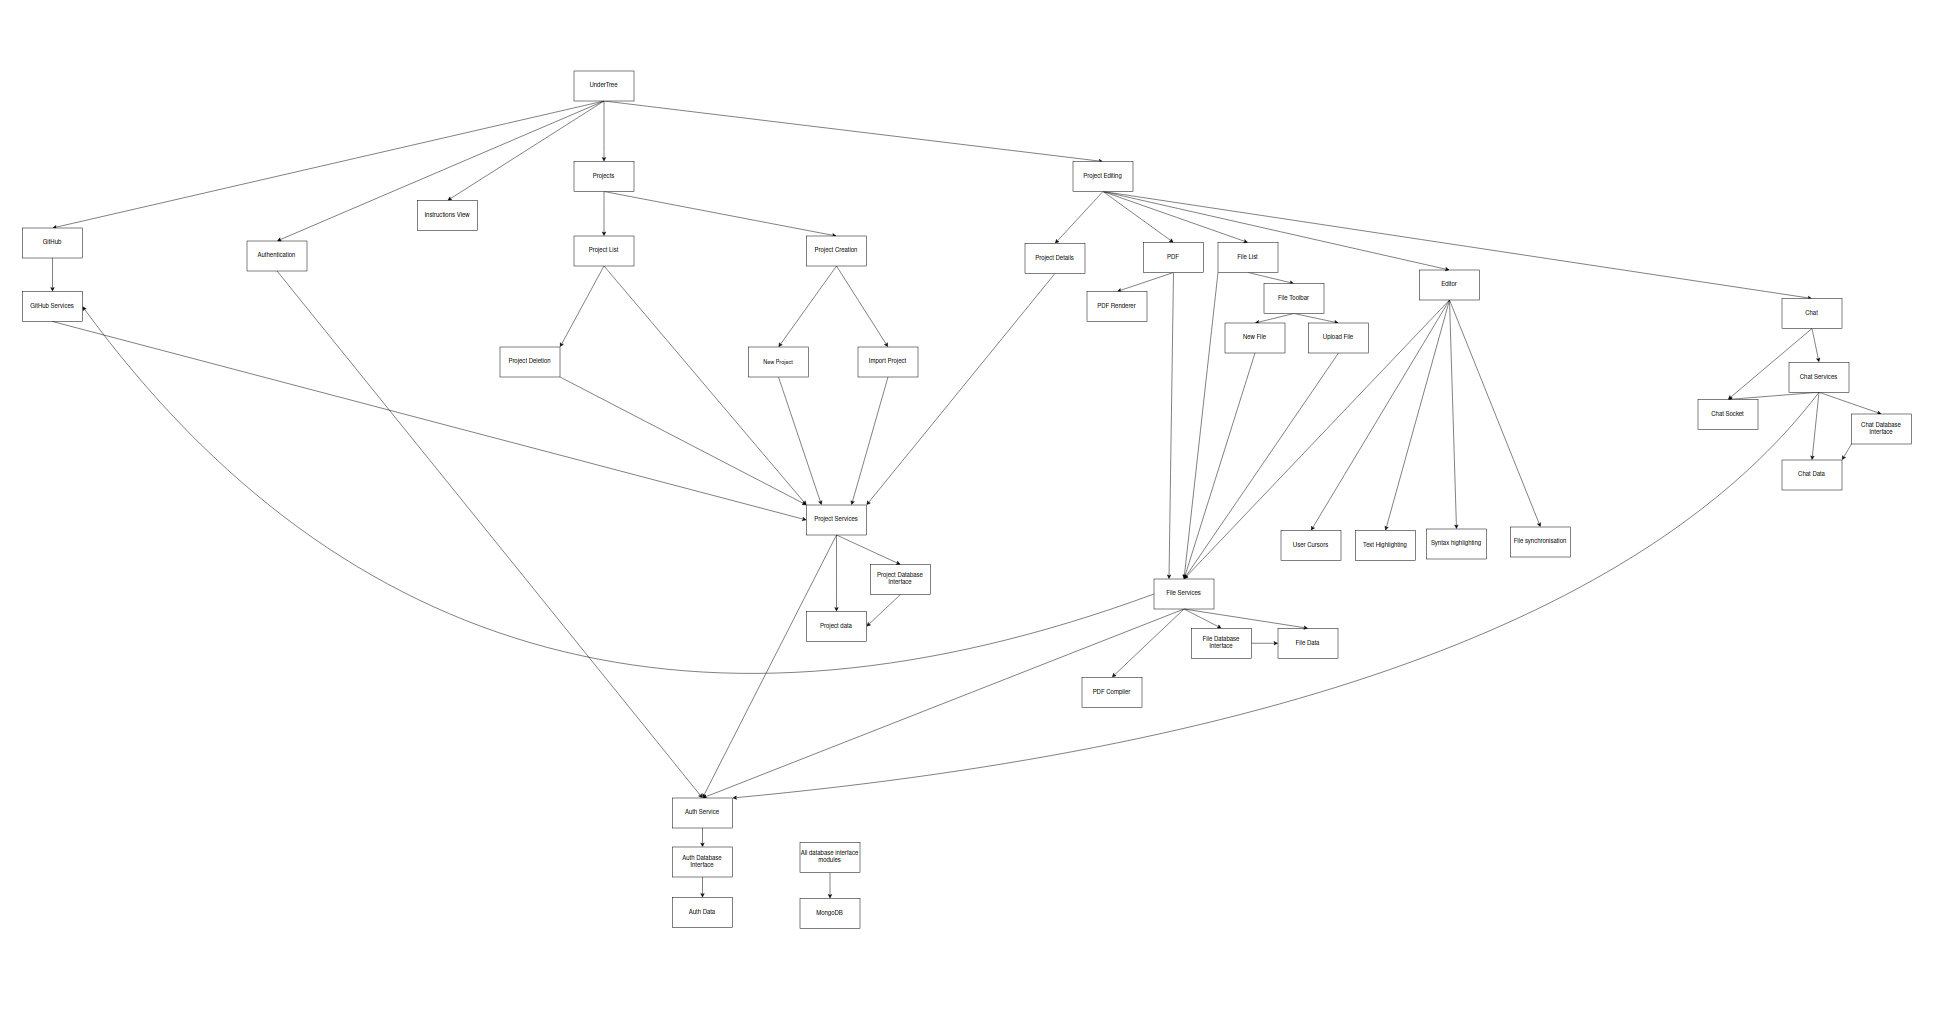
\includegraphics[width=0.9\textwidth]{mgdiagram.png}
	\caption{Use hierarchy among modules \href{mgdiagram.png}{Image source}}
	\label{FigUH}
\end{figure}

%\section*{References}

\bibliographystyle {plainnat}
\bibliography{../../../refs/References}

\end{document}